% This LaTeX was auto-generated from MATLAB code.
% To make changes, update the MATLAB code and export to LaTeX again.

\documentclass{article}

\usepackage[utf8]{inputenc}
\usepackage[T1]{fontenc}
\usepackage{lmodern}
\usepackage{graphicx}
\usepackage{color}
\usepackage{hyperref}
\usepackage{amsmath}
\usepackage{amsfonts}
\usepackage{epstopdf}
\usepackage[table]{xcolor}
\usepackage{matlab}

\sloppy
\epstopdfsetup{outdir=./}
\graphicspath{ {./Lagrangian_sim_images/} }

\begin{document}

\begin{matlabcode}
clc; clear; close all;
\end{matlabcode}

\begin{par}
\begin{flushleft}
Loading test data for pendulum drops:
\end{flushleft}
\end{par}

\begin{matlabcode}

load("data\PendTest.mat");
%Cleaning up
pendTest.data_1.angle(1:round(0.12*250)) = [];
pendTest.data_1.time(1:round(0.12*250)) = [];
pendTest.data_1.angle = pendTest.data_1.angle(:) - pendTest.data_1.angle(1);
pendTest.data_1.time = pendTest.data_1.time(:) - pendTest.data_1.time(1);
\end{matlabcode}

\begin{par}
\begin{flushleft}
 Parameters for matematical model
\end{flushleft}
\end{par}

\begin{matlabcode}
l_B = 0.132; % [m] Base langth. 13.2cm measured. 
l_P = 0.21; % [m] Pendulum length. 24cm measured.
I_B = 2.1*(1/12)*0.05*0.25^2; % [kg*m^2]Base, motor ang gerbox inertia (about mass centre)
I_P = (1/3)*0.010*0.25^2*1; % [kg*m^2] Pendulum inertia (about mass centre). Estimated with mass = 10g
m_P = 0.026 * 1; % [kg] Pendulum mass. 26g measured
B_B = -0.00048*3;%0.01; % [Nm*rad/s] Motor friction.
B_P = -0.00048; % [Nm*rad/s] Penulum friction.
g = 9.81; % [m/s^2] gravity.

%Motor parameters
L = 1.3/1000 * 1;; % [Henry] Motor inductance. From random data sheet
R = 5; % [Omh] Motor resistance. From random data sheet
K_t = 0.089240515 ; % [Nm/A] Motor tourqe constant. From random data sheet
K_e = 0.089240515 * 0.7; % [V/(rad/s)] Motor back EMF constant. From random data sheet
\end{matlabcode}

\begin{par}
\begin{flushleft}
 LQR
\end{flushleft}
\end{par}

\begin{matlabcode}

A_lqr = [
    0, 1, 0, 0, 0; 
    (g*m_P*(m_P*l_B^2 + I_B))/(I_P*m_P*l_B^2 + I_B*m_P*l_P^2 + I_B*I_P), (B_P*(m_P*l_B^2 + l_P*m_P*l_B + I_B))/(I_P*m_P*l_B^2 + I_B*m_P*l_P^2 + I_B*I_P), 0, -(B_B*l_B*l_P*m_P)/(I_P*m_P*l_B^2 + I_B*m_P*l_P^2 + I_B*I_P), -(K_t*l_B*l_P*m_P)/(I_P*m_P*l_B^2 + I_B*m_P*l_P^2 + I_B*I_P); 
    0, 0, 0, 1, 0; 
    -(g*l_B*l_P*m_P^2)/(I_P*m_P*l_B^2 + I_B*m_P*l_P^2 + I_B*I_P), -(B_P*(m_P*l_P^2 + l_B*m_P*l_P + I_P))/(I_P*m_P*l_B^2 + I_B*m_P*l_P^2 + I_B*I_P), 0, (B_B*(m_P*l_P^2 + I_P))/(I_P*m_P*l_B^2 + I_B*m_P*l_P^2 + I_B*I_P), (K_t*(m_P*l_P^2 + I_P))/(I_P*m_P*l_B^2 + I_B*m_P*l_P^2 + I_B*I_P); 
    0, 0, 0, -K_e/L, -R/L];

B = [0; 0; 0; 0; 1/L];

Q_lqr = [100 0 0 0 0;
    0 10 0 0 0;
    0 0 1 0 0;
    0 0 0 1 0
    0 0 0 0 1];

R_lqr = 0.5;

K_lqr = lqr(A_lqr, B, Q_lqr, R_lqr);
\end{matlabcode}

\begin{par}
\begin{flushleft}
Creating function handler for functions, this setts the parameters. One with locked base and on with free base.
\end{flushleft}
\end{par}

\begin{matlabcode}
odeFunHandler_Locked = @(t, x) odeFun_BaseLock(x, l_B, l_P, I_B, I_P, L, m_P, B_B, B_P, R, g, K_t, K_e, K_lqr, B)
\end{matlabcode}
\begin{matlaboutput}
odeFunHandler_Locked = 
    @(t,x)odeFun_BaseLock(x,l_B,l_P,I_B,I_P,L,m_P,B_B,B_P,R,g,K_t,K_e,K_lqr,B)

\end{matlaboutput}
\begin{matlabcode}
odeFunHandler_Free = @(t, x) odeFun_BaseFree(x, l_B, l_P, I_B, I_P, L, m_P, B_B, B_P, R, g, K_t, K_e, K_lqr, B)
\end{matlabcode}
\begin{matlaboutput}
odeFunHandler_Free = 
    @(t,x)odeFun_BaseFree(x,l_B,l_P,I_B,I_P,L,m_P,B_B,B_P,R,g,K_t,K_e,K_lqr,B)

\end{matlaboutput}
\begin{matlabcode}
odeFunHandler_NoPendulum= @(t, x) odeFun_NoPendulum(t, x, l_B, l_P, I_B, I_P, L, m_P, B_B, B_P, R, g, K_t, K_e, K_lqr, B)
\end{matlabcode}
\begin{matlaboutput}
odeFunHandler_NoPendulum = 
    @(t,x)odeFun_NoPendulum(t,x,l_B,l_P,I_B,I_P,L,m_P,B_B,B_P,R,g,K_t,K_e,K_lqr,B)

\end{matlaboutput}
\begin{matlabcode}
odeFunHandler_impulseTest= @(t, x) odeFun_impulseTest(t, x, l_B, l_P, I_B, I_P, L, m_P, B_B, B_P, R, g, K_t, K_e, K_lqr, B)
\end{matlabcode}
\begin{matlaboutput}
odeFunHandler_impulseTest = 
    @(t,x)odeFun_impulseTest(t,x,l_B,l_P,I_B,I_P,L,m_P,B_B,B_P,R,g,K_t,K_e,K_lqr,B)

\end{matlaboutput}

\begin{par}
\begin{flushleft}
Simulate from -pi/2. Locked base.
\end{flushleft}
\end{par}

\begin{matlabcode}
disp(pendTest.data_1.description)
\end{matlabcode}
\begin{matlaboutput}
Dropped from pi/2. Base is locked
\end{matlaboutput}
\begin{matlabcode}
% For Runge-Kutta solver
tspan = [0 5];
% Initial condition
x0 = [
    -1.528;
    0;
    0;
    0;
    0];

%  Runge-Kutta solver
[t, x] = ode45(odeFunHandler_Locked, tspan, x0);

% Plotting:
plot(t, x(:, 1), LineWidth=2);
title('Pendulum angle. ' + pendTest.data_1.description);
ylabel('Angle [rad]');
xlabel('time [s]');
hold on
%plot(data1.pendFirst.time, data1.pendFirst.angle - pi/2+0.05,LineWidth=2);
plot(pendTest.data_1.time, pendTest.data_1.angle - pi/2+0.05, LineWidth=2);
xaxis(tspan)
legend('Mathematical model', 'Physical model');
grid on
box on
hold off
\end{matlabcode}
\begin{center}
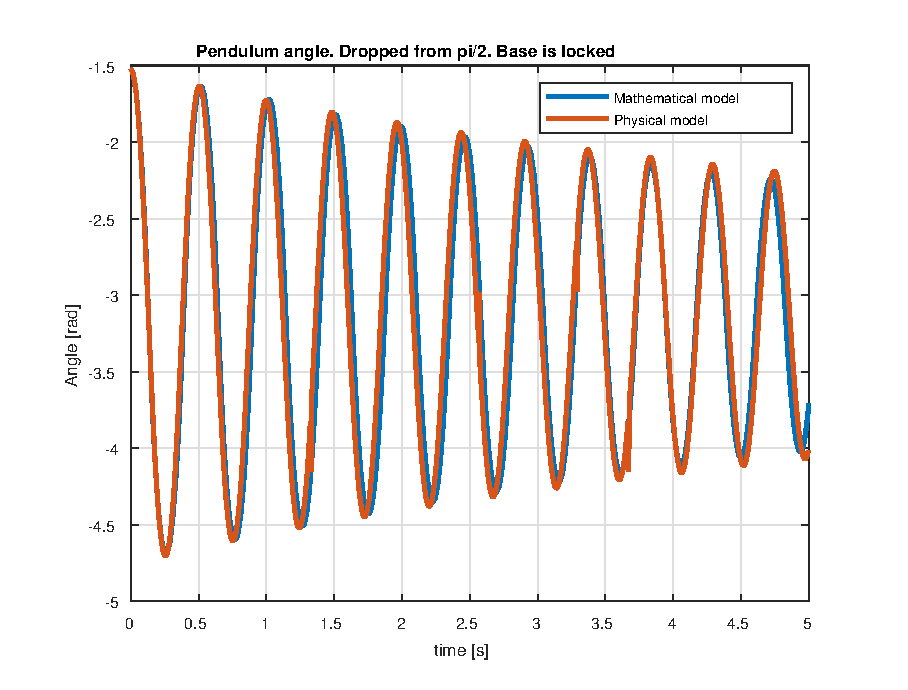
\includegraphics[width=\maxwidth{56.196688409433015em}]{figure_0.eps}
\end{center}

\begin{par}
\begin{flushleft}
Simulate from pi/2. Locked base.
\end{flushleft}
\end{par}

\begin{matlabcode}
disp(pendTest.data_2.description)
\end{matlabcode}
\begin{matlaboutput}
Dropped from -pi/2. Base is locked
\end{matlaboutput}
\begin{matlabcode}
% For Runge-Kutta solver
tspan = [0 5];
% Initial condition
x0 = [
    1.63;
    0;
    0;
    0;
    0];

%  Runge-Kutta solver
[t, x] = ode45(odeFunHandler_Locked, tspan, x0);

% Plotting:
plot(t, x(:, 1), LineWidth=2);
title('Pendulum angle. ' + pendTest.data_2.description);
ylabel('Angle [rad]');
xlabel('time [s]');
hold on
plot(pendTest.data_2.time, pendTest.data_2.angle + pi/2+0.05, LineWidth=2);
xaxis(tspan)
legend('Mathematical model', 'Physical model');
grid on
box on
hold off
\end{matlabcode}
\begin{center}
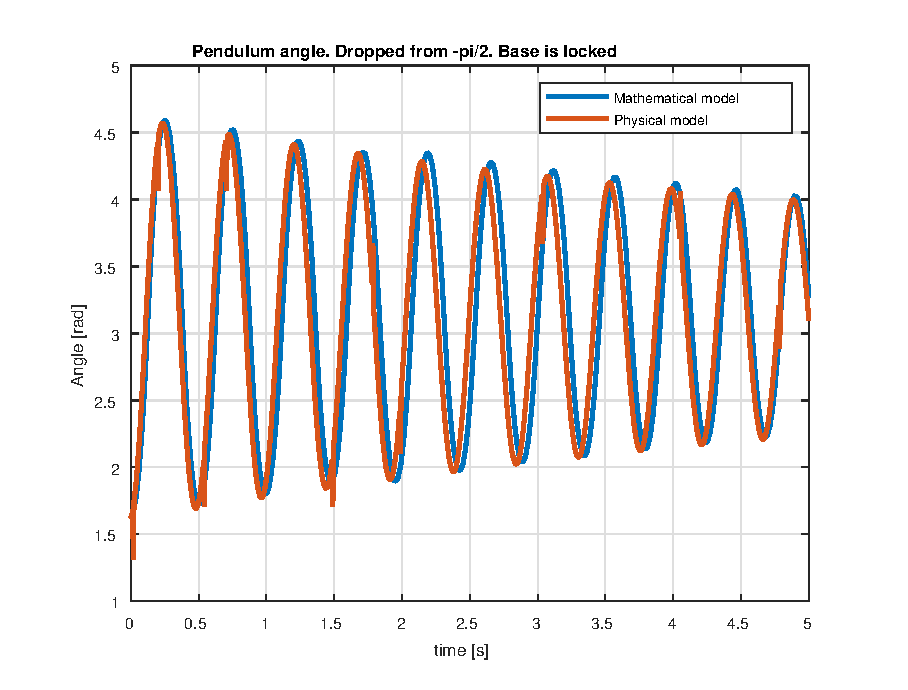
\includegraphics[width=\maxwidth{56.196688409433015em}]{figure_1.eps}
\end{center}

\begin{par}
\begin{flushleft}
Simulate from - pi/2. Base is free
\end{flushleft}
\end{par}

\begin{matlabcode}
disp(pendTest.data_3.description)
\end{matlabcode}
\begin{matlaboutput}
Dropped from pi/2. Base is free
\end{matlaboutput}
\begin{matlabcode}
% For Runge-Kutta solver
tspan = [0 5];
% Initial condition
x0 = [
    -1.528;
    0;
    0;
    0;
    0];

%  Runge-Kutta solver
[t, x] = ode45(odeFunHandler_Free, tspan, x0);

% Plotting:
plot(t, x(:, 1), LineWidth=2);
title('Pendulum angle. ' + pendTest.data_3.description);
ylabel('Angle [rad]');
xlabel('time [s]');
hold on
plot(pendTest.data_3.time, pendTest.data_3.angle - pi/2+0.05,LineWidth=2);
legend('Mathematical model', 'Physical model');
xaxis(tspan)
grid on
box on
hold off
\end{matlabcode}
\begin{center}
\includegraphics[width=\maxwidth{56.196688409433015em}]{figure_2.eps}
\end{center}
\begin{matlabcode}


plot(t, x(:, 3), LineWidth=2);
title('\theta_b')
title('Base angle' + pendTest.data_3.description)
xlabel('time [s]');
hold on
plot(pendTest.data_3.time, pendTest.data_3.baseAngle*(-1) -0.21788, LineWidth=2); %NB inverted
xaxis(tspan)
hold off
\end{matlabcode}
\begin{center}
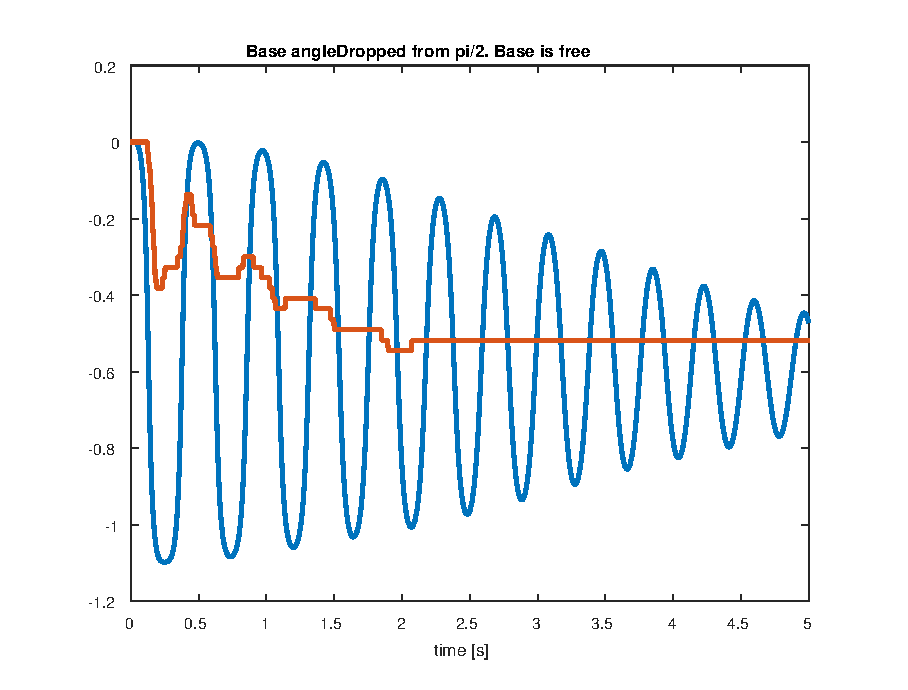
\includegraphics[width=\maxwidth{56.196688409433015em}]{figure_3.eps}
\end{center}

\begin{par}
\begin{flushleft}
Simulate from - pi/2. Base is free
\end{flushleft}
\end{par}

\begin{matlabcode}
disp(pendTest.data_4.description)
\end{matlabcode}
\begin{matlaboutput}
Dropped from -pi/2. Base is free
\end{matlaboutput}
\begin{matlabcode}
% For Runge-Kutta solver
tspan = [0 5];
% Initial condition
x0 = [
    1.528;
    0;
    0;
    0;
    0];

%  Runge-Kutta solver
[t, x] = ode45(odeFunHandler_Free, tspan, x0);

% Plotting:
plot(t, x(:, 1), LineWidth=2);
title('Pendulum angle. ' + pendTest.data_4.description);
ylabel('Angle [rad]');
xlabel('time [s]');
hold on
plot(pendTest.data_4.time, pendTest.data_4.angle + pi/2+0.05*0,LineWidth=2);
xaxis(tspan)
legend('Mathematical model', 'Physical model');
grid on
box on
hold off
\end{matlabcode}
\begin{center}
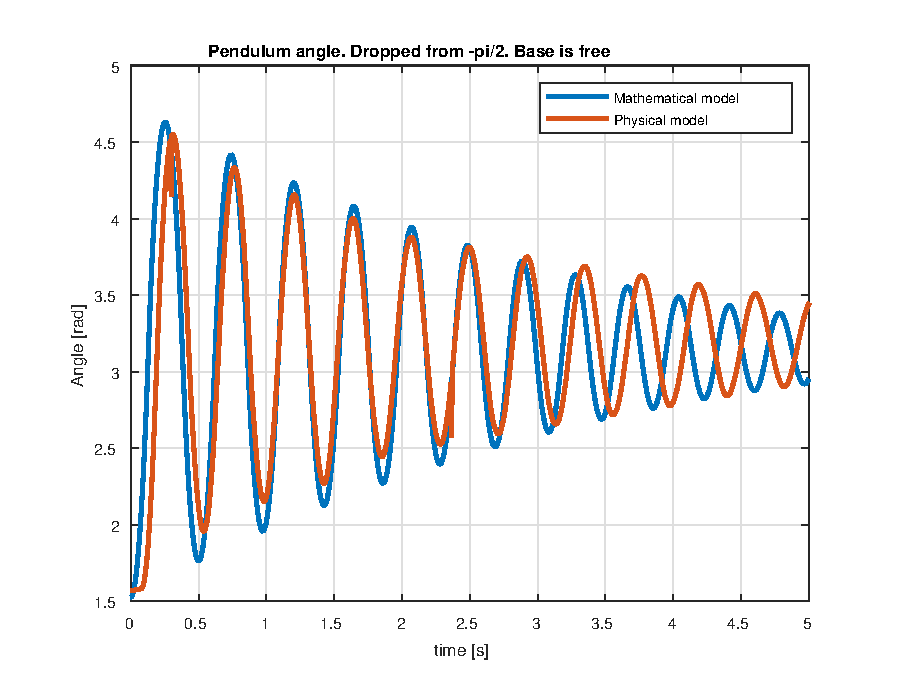
\includegraphics[width=\maxwidth{56.196688409433015em}]{figure_4.eps}
\end{center}
\begin{matlabcode}


plot(t, x(:, 3), LineWidth=2);
title('Base angle. ' + pendTest.data_4.description)
ylabel('Angle [rad]');
xlabel('time [s]');
hold on
plot(pendTest.data_4.time, pendTest.data_4.baseAngle*(-1) + 0.354, LineWidth=2); %NB inverted
xaxis(tspan)
hold off
\end{matlabcode}
\begin{center}
\includegraphics[width=\maxwidth{56.196688409433015em}]{figure_5.eps}
\end{center}


\begin{par}
\begin{flushleft}
Testing the base without pendulum
\end{flushleft}
\end{par}

\begin{matlabcode}

load("data\BaseTest.mat");
% For Runge-Kutta solver
tspan = [0 25];
% Initial condition
x0 = [
    0;
    0;
    0;
    0;
    0];


%  Runge-Kutta solver
[t, x] = ode45(odeFunHandler_NoPendulum, tspan, x0);
%y = lowpass(x,fpass,fs) specifies that x has been sampled at a rate of fs hertz. fpass is the passband frequency of the filter in hertz.
x(:, 4) = lowpass(x(:, 4), 10/(2*pi), 250);

plot(t, x(:, 4), LineWidth=2)
title('Base angle vel. No pendulum')
ylabel('Angle vel [rad/s]');
xlabel('time [s]');
hold on
plot(BaseTest.baseAngleVelFilterd.time, BaseTest.baseAngleVelFilterd.signals.values,LineWidth=2)
legend('Mathematical model', 'Physical model');
hold off
\end{matlabcode}
\begin{center}
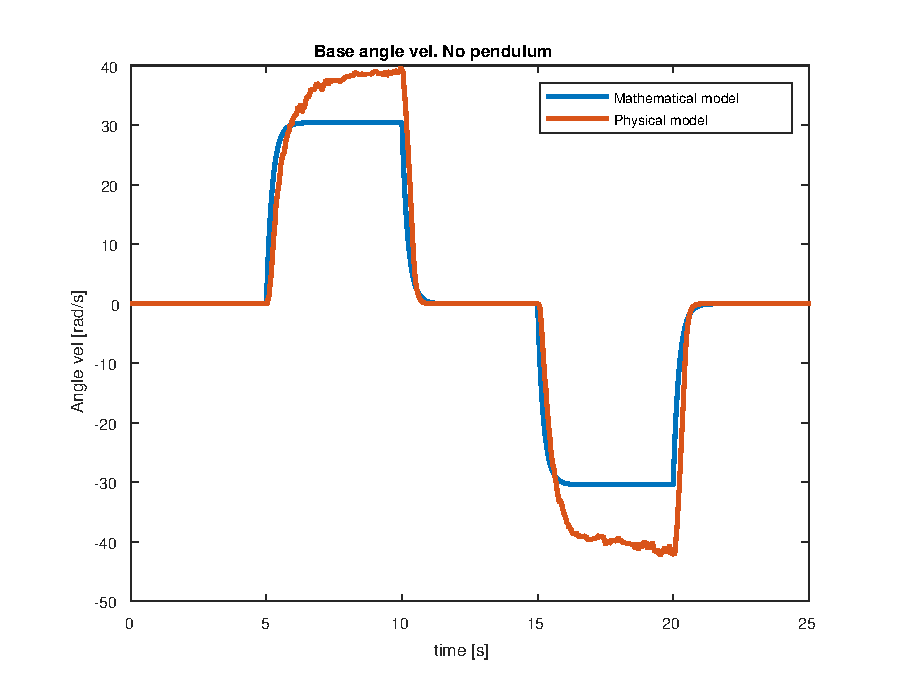
\includegraphics[width=\maxwidth{56.196688409433015em}]{figure_6.eps}
\end{center}
\begin{matlabcode}

plot(t, x(:, 3), LineWidth=2)
title('Base angle. No pendulum')
ylabel('Angle [rad]');
xlabel('time [s]');
hold on
plot(BaseTest.baseAngle.time, BaseTest.baseAngle.signals.values,LineWidth=2)
legend('Mathematical model', 'Physical model');
hold off 
\end{matlabcode}
\begin{center}
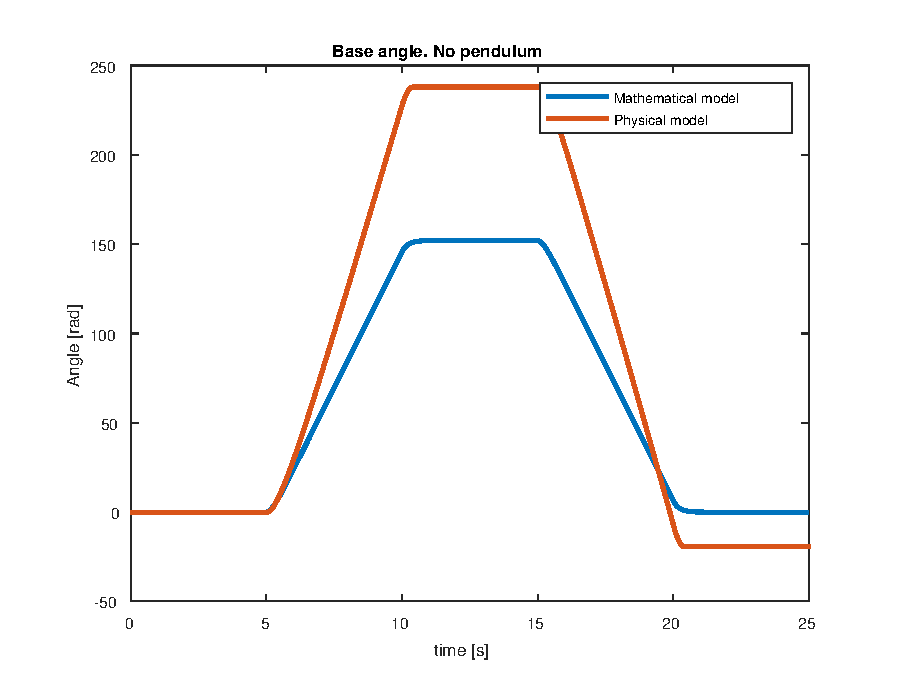
\includegraphics[width=\maxwidth{56.196688409433015em}]{figure_7.eps}
\end{center}
\begin{matlabcode}

\end{matlabcode}


\begin{par}
\begin{flushleft}
\textit{Impulse test}
\end{flushleft}
\end{par}

\begin{matlabcode}
load("data\impulsTest100.mat");
disp(impulseTest.description)
\end{matlabcode}
\begin{matlaboutput}
Impulse test. Impuls after 0.5s. Ampludude =100/255. Duration = 0.5s. Then 15 seconds of rest.
\end{matlaboutput}
\begin{matlabcode}
% For Runge-Kutta solver
tspan = [0 16];
% Initial condition
x0 = [
    pi;
    0;
    0;
    0;
    0];

%  Runge-Kutta solver
[t, x] = ode45(odeFunHandler_impulseTest, tspan, x0);


plot(t, x(:, 3), LineWidth=2)
title('Base angle')
ylabel('Angle [rad]');
xlabel('time [s]');
hold on
plot(impulseTest.baseAngle.time, impulseTest.baseAngle.signals.values,LineWidth=2)
legend('Mathematical model', 'Physical model');
hold off;
\end{matlabcode}
\begin{center}
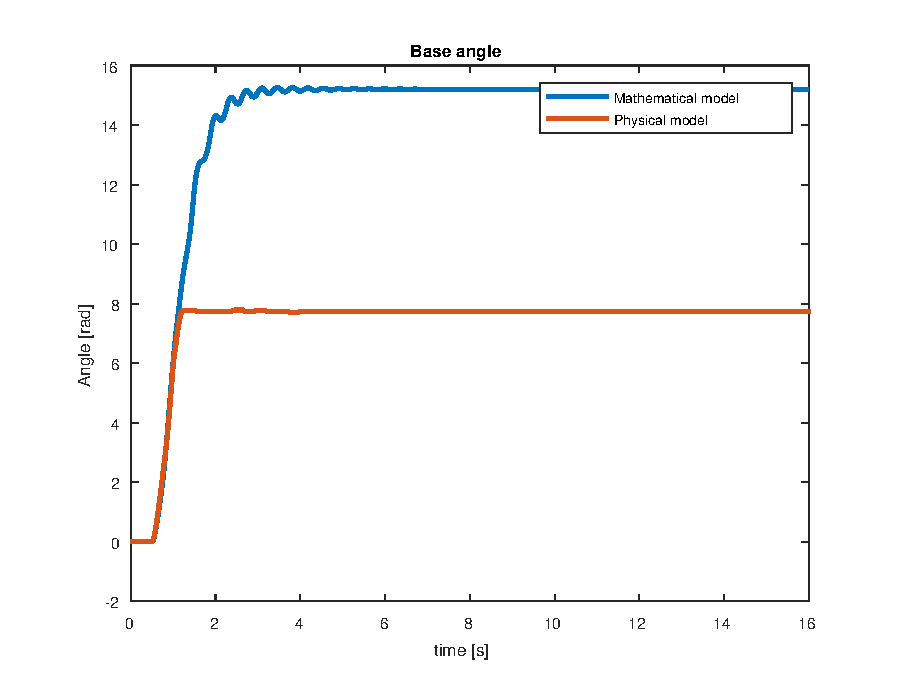
\includegraphics[width=\maxwidth{56.196688409433015em}]{figure_8.eps}
\end{center}
\begin{matlabcode}


plot(t, x(:, 4), LineWidth=2)
title('Base angle vel')
ylabel('Angle [rad/s]');
xlabel('time [s]');
hold on
plot(impulseTest.baseAngleVelFilterd.time, impulseTest.baseAngleVelFilterd.signals.values,LineWidth=2)
legend('Mathematical model', 'Physical model');
hold off;
\end{matlabcode}
\begin{center}
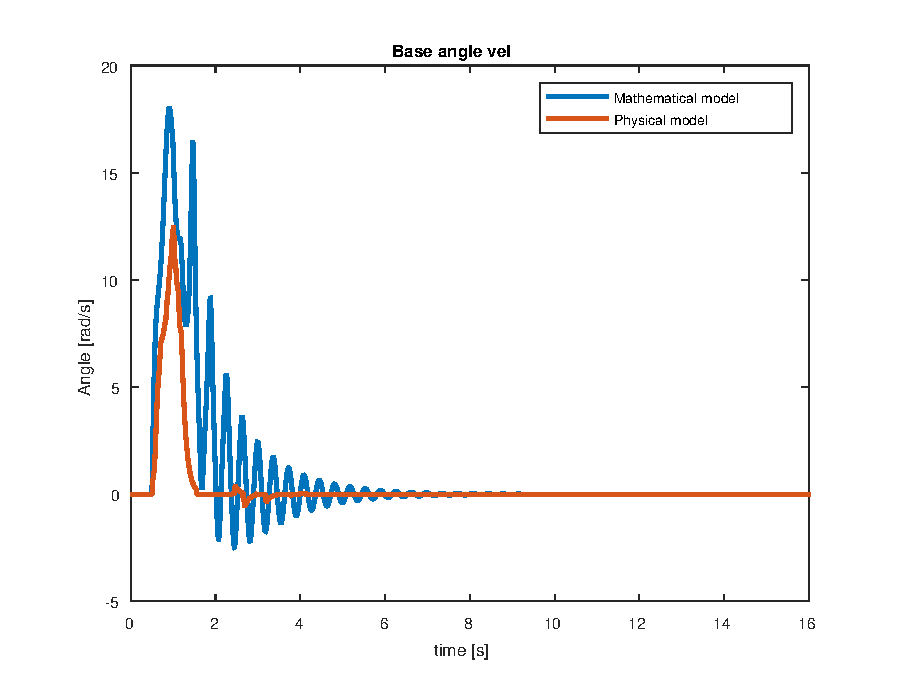
\includegraphics[width=\maxwidth{56.196688409433015em}]{figure_9.eps}
\end{center}
\begin{matlabcode}

plot(t, x(:, 1), LineWidth=2)
title('Pend angle')
ylabel('Angle [rad]');
xlabel('time [s]');
hold on
plot(impulseTest.pendAngle.time, (-1)*impulseTest.pendAngle.signals.values + pi,LineWidth=2) %NB inveted
legend('Mathematical model', 'Physical model'); 
hold off
\end{matlabcode}
\begin{center}
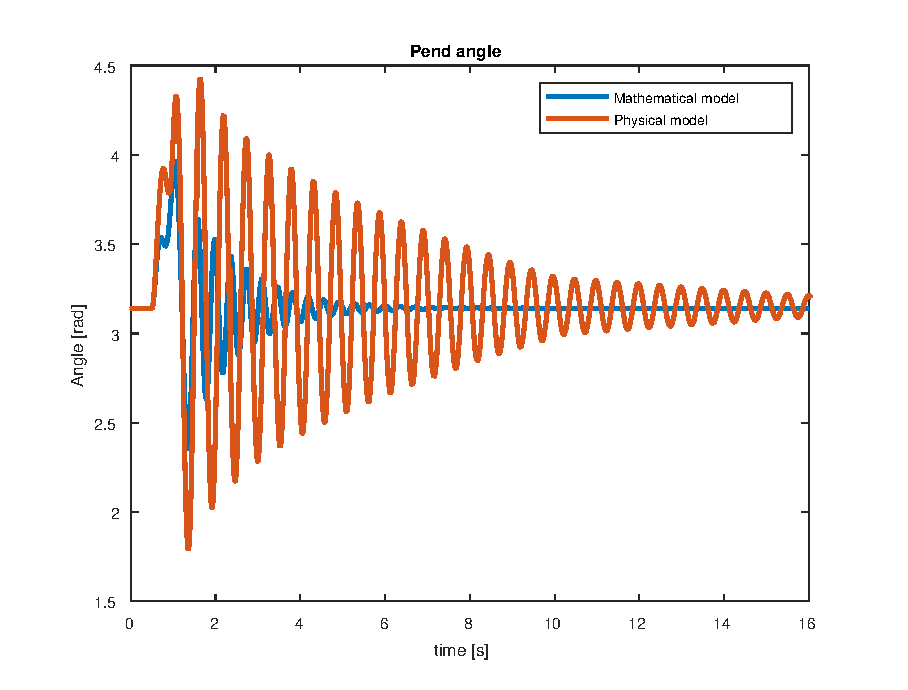
\includegraphics[width=\maxwidth{56.196688409433015em}]{figure_10.eps}
\end{center}
\begin{matlabcode}

plot(t, x(:, 5), LineWidth=2)
\end{matlabcode}
\begin{center}
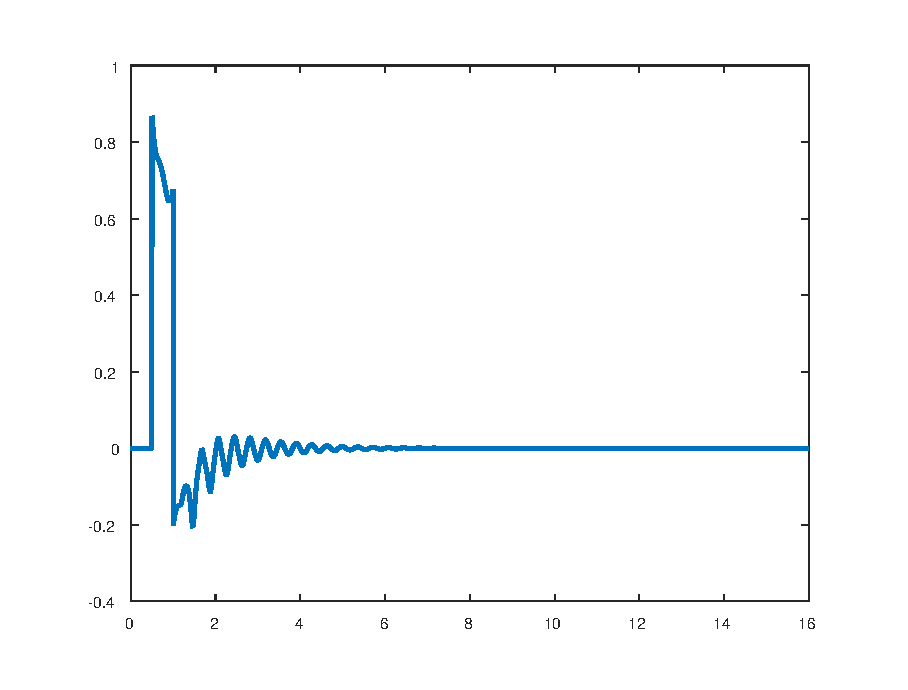
\includegraphics[width=\maxwidth{56.196688409433015em}]{figure_11.eps}
\end{center}
\begin{matlabcode}

\end{matlabcode}


\begin{matlabcode}
%odeFun_NoPendulum(0, [pi/2; 0; 0; 0; 0;], l_B, l_P, I_B, I_P, L, m_P, B_B, B_P, R, g, K_t, K_e, K_lqr, B)
\end{matlabcode}


\begin{matlabcode}
function dxdt = odeFun_BaseLock(x, l_B, l_P, I_B, I_P, L, m_P, B_B, B_P, R, g, K_t, K_e, K_lqr, B)
    dxdt = [
    x(2); 
    -(B_P*x(2) + g*m_P*sin(x(1)) + l_P^2*m_P*cos(x(1))*sin(x(1))*x(4)^2 - (l_B*l_P*m_P*cos(x(1))*(- m_P*sin(2*x(1))*x(4)*l_P^2*x(2) + l_B*m_P*sin(x(1))*l_P*x(2)^2 - B_P*x(2) + B_B*x(4) + K_t*x(5)))/(m_P*l_B^2 - m_P*l_P^2*cos(x(1))^2 + m_P*l_P^2 + I_B))/((m_P*l_P^2 + I_P)*((l_B^2*l_P^2*m_P^2*cos(x(1))^2)/((m_P*l_P^2 + I_P)*(m_P*l_B^2 - m_P*l_P^2*cos(x(1))^2 + m_P*l_P^2 + I_B)) - 1)); 
    x(4); 
    -(B_B*x(4) - B_P*x(2) + K_t*x(5) - l_P^2*m_P*sin(2*x(1))*x(4)*x(2) + l_B*l_P*m_P*sin(x(1))*x(2)^2 - (l_B*l_P*m_P*cos(x(1))*(m_P*cos(x(1))*sin(x(1))*l_P^2*x(4)^2 + B_P*x(2) + g*m_P*sin(x(1))))/(m_P*l_P^2 + I_P))/(((l_B^2*l_P^2*m_P^2*cos(x(1))^2)/((m_P*l_P^2 + I_P)*(m_P*l_B^2 - m_P*l_P^2*cos(x(1))^2 + m_P*l_P^2 + I_B)) - 1)*(m_P*l_B^2 - m_P*l_P^2*cos(x(1))^2 + m_P*l_P^2 + I_B)); 
    -(K_e*x(4) - 0 + R*x(5))/L
    ];
dxdt(5) = 0; % Setting current to 0
dxdt(3:4) = 0; % Locking base
end

function dxdt = odeFun_BaseFree(x, l_B, l_P, I_B, I_P, L, m_P, B_B, B_P, R, g, K_t, K_e, K_lqr, B)
    dxdt = [
    x(2); 
    -(B_P*x(2) + g*m_P*sin(x(1)) + l_P^2*m_P*cos(x(1))*sin(x(1))*x(4)^2 - (l_B*l_P*m_P*cos(x(1))*(- m_P*sin(2*x(1))*x(4)*l_P^2*x(2) + l_B*m_P*sin(x(1))*l_P*x(2)^2 - B_P*x(2) + B_B*x(4) + K_t*x(5)))/(m_P*l_B^2 - m_P*l_P^2*cos(x(1))^2 + m_P*l_P^2 + I_B))/((m_P*l_P^2 + I_P)*((l_B^2*l_P^2*m_P^2*cos(x(1))^2)/((m_P*l_P^2 + I_P)*(m_P*l_B^2 - m_P*l_P^2*cos(x(1))^2 + m_P*l_P^2 + I_B)) - 1)); 
    x(4); 
    -(B_B*x(4) - B_P*x(2) + K_t*x(5) - l_P^2*m_P*sin(2*x(1))*x(4)*x(2) + l_B*l_P*m_P*sin(x(1))*x(2)^2 - (l_B*l_P*m_P*cos(x(1))*(m_P*cos(x(1))*sin(x(1))*l_P^2*x(4)^2 + B_P*x(2) + g*m_P*sin(x(1))))/(m_P*l_P^2 + I_P))/(((l_B^2*l_P^2*m_P^2*cos(x(1))^2)/((m_P*l_P^2 + I_P)*(m_P*l_B^2 - m_P*l_P^2*cos(x(1))^2 + m_P*l_P^2 + I_B)) - 1)*(m_P*l_B^2 - m_P*l_P^2*cos(x(1))^2 + m_P*l_P^2 + I_B)); 
    -(K_e*x(4) - 0 + R*x(5))/L
    ];
dxdt(5) = 0; % Setting current to 0
end

function dxdt = odeFun_NoPendulum(t, x, l_B, l_P, I_B, I_P, L, m_P, B_B, B_P, R, g, K_t, K_e, K_lqr, B)
l_P=0;
I_P=0;
m_P=0;
B_P=0;

U = 0;
V = 11.1;
if(t >= 5 && t <=10)
    U = V*100/255;
elseif(t >=15 && t <=20)
    U = V*(-100)/255;
else
    U = 0;
end
dxdt = [
    x(2);
    -(B_P*x(2) + g*m_P*sin(x(1)) + l_P^2*m_P*cos(x(1))*sin(x(1))*x(4)^2 - (l_B*l_P*m_P*cos(x(1))*(- m_P*sin(2*x(1))*x(4)*l_P^2*x(2) + l_B*m_P*sin(x(1))*l_P*x(2)^2 - B_P*x(2) + B_B*x(4) + K_t*x(5)))/(m_P*l_B^2 - m_P*l_P^2*cos(x(1))^2 + m_P*l_P^2 + I_B))/((m_P*l_P^2 + I_P)*((l_B^2*l_P^2*m_P^2*cos(x(1))^2)/((m_P*l_P^2 + I_P)*(m_P*l_B^2 - m_P*l_P^2*cos(x(1))^2 + m_P*l_P^2 + I_B)) - 1));
    x(4);
    %-(B_B*x(4) - B_P*x(2) + K_t*x(5) - l_P^2*m_P*sin(2*x(1))*x(4)*x(2) + l_B*l_P*m_P*sin(x(1))*x(2)^2 - (l_B*l_P*m_P*cos(x(1))*(m_P*cos(x(1))*sin(x(1))*l_P^2*x(4)^2 + B_P*x(2) + g*m_P*sin(x(1))))/(m_P*l_P^2 + I_P))/(((l_B^2*l_P^2*m_P^2*cos(x(1))^2)/((m_P*l_P^2 + I_P)*(m_P*l_B^2 - m_P*l_P^2*cos(x(1))^2 + m_P*l_P^2 + I_B)) - 1)*(m_P*l_B^2 - m_P*l_P^2*cos(x(1))^2 + m_P*l_P^2 + I_B));
    (K_t*x(5)+B_B*x(4))/I_B;
    -(K_e*x(4) - 0 + R*x(5))/L
    ];
dxdt(1:2) = 0;
dxdt = dxdt + B*U;
end

function dxdt = odeFun_impulseTest(t, x, l_B, l_P, I_B, I_P, L, m_P, B_B, B_P, R, g, K_t, K_e, K_lqr, B)
U = 0;
V = 11.1;

if(t >= 0.5)
    U = V*(100/255);
end
if(t > 1.0)
    U = 0;
end

dxdt = [
    x(2);
    -(B_P*x(2) + g*m_P*sin(x(1)) + l_P^2*m_P*cos(x(1))*sin(x(1))*x(4)^2 - (l_B*l_P*m_P*cos(x(1))*(- m_P*sin(2*x(1))*x(4)*l_P^2*x(2) + l_B*m_P*sin(x(1))*l_P*x(2)^2 - B_P*x(2) + B_B*x(4) + K_t*x(5)))/(m_P*l_B^2 - m_P*l_P^2*cos(x(1))^2 + m_P*l_P^2 + I_B))/((m_P*l_P^2 + I_P)*((l_B^2*l_P^2*m_P^2*cos(x(1))^2)/((m_P*l_P^2 + I_P)*(m_P*l_B^2 - m_P*l_P^2*cos(x(1))^2 + m_P*l_P^2 + I_B)) - 1));
    x(4);
    -(B_B*x(4) - B_P*x(2) + K_t*x(5) - l_P^2*m_P*sin(2*x(1))*x(4)*x(2) + l_B*l_P*m_P*sin(x(1))*x(2)^2 - (l_B*l_P*m_P*cos(x(1))*(m_P*cos(x(1))*sin(x(1))*l_P^2*x(4)^2 + B_P*x(2) + g*m_P*sin(x(1))))/(m_P*l_P^2 + I_P))/(((l_B^2*l_P^2*m_P^2*cos(x(1))^2)/((m_P*l_P^2 + I_P)*(m_P*l_B^2 - m_P*l_P^2*cos(x(1))^2 + m_P*l_P^2 + I_B)) - 1)*(m_P*l_B^2 - m_P*l_P^2*cos(x(1))^2 + m_P*l_P^2 + I_B));
    %(K_t*x(5)+B_B*x(4))/I_B;
    -(K_e*x(4) - 0 + R*x(5))/L
    ];

dxdt = dxdt + B*U;

end
\end{matlabcode}

\end{document}
